\section{Motivation}

The FINken project aims to create a swarm of autonomously flying quadcopters to research swarm intelligence beheaviour on robots.
Many algorithms in swarm intelligence are based on distance values. \todo{source}
On this occasion it is important to find a sensor that is capable to measure distances and to integrate it into the FINken robots.
An obvious choice for this distance is measuring the spacial distance in between the robots\footnote{
The mathematical distance-property might not actually need to be something as close to a physical property, but it is beneficial to be able to measure and watch the robots interacting with their physical environment.}.

\todo{establish type of ranging (node <-> node)}

\section{Requirements}
\label{req}
There are basically three requirements for the ranging sensor.
Those requirements will act as a base to choose and to evaluate the new sensor.

\begin{enumerate}
	\item interaction between the copter and the ranging modules shall be minimal
	\item the ranging nodes need to be integrated into the copter
	\item the values yielded by ranging shall be of usable quality
\end{enumerate}

\subsection{Interaction between Copter and Ranging}
\label{req1}
The copter shall not influence the function of the ranging modules and vice versa.
I.e. using an ultrasonic ranging method might not be feasible as the copter already uses multiple ultrasonic sensors.
If no measures are taken to counteract medium access problems both sensors will disrupt each other to a point where the sensor values of both sensors are completely useless.

This requirements might be watered down to a certain degree.
If there is interaction between copter and ranging sensors the setup of the quadcopter might be changed to eliminate the interaction.
However the FINken robot is beeing used in research and changing one component usually means almost all components have to be touched as well, as most components are interdependable to some degree.\todo{wording}

\subsection{Integration of the Ranging Modules}
\label{req2}
In order to be used in the FINken project the sensors need to be integrated into the robots.
This means the ranging modules need to be lightweight and small enough to fit on a flying robot.
Additionally there needs to be an interface that can transmit the data from the new sensor to the firmware controlling the robot.

One of the aspects of integration is that the robots shall interact locally to form a swarm in contrast to multi agent systems that rely on global information.
As a consequence measuring the positions of the copters with an external sensors and providing the distances via telemetry is not sufficient—the robots shall not be dependant on external sensors.

\subsection{Yielding Usefull Values}
\label{req3}
Yielding usefull values seems to be a trivial requirement, but is actually the hardest of all three.
The area of operation for the FINken robots is only \SI{3}{m} by \SI{4}{m} so the range measurements need to be pretty accurate for small distances. \todo{provide metric for hypothesis}
Additionally the update frequency needs to be quite high as the copters are able to move with great accelarations and velocities.
\todo{moar!}

\section{The FINken Robot Platform}


Goal of the FINken project is to implement intelligent swarm beheaviour on flying robots and research how swarm collaboration works in a real world application.
The robots need to fly in an stable manner on their own and be capable of interacting without disrupting the operation of the other swarm members.
Those robots shall perform given tasks defined to encurage swarm based interaction, their beheaviour can be evaluated and compared to the theoretical models developed by swarm intelligence research.

\subsection{Robot Description}
\begin{figure}[H]
	\centering
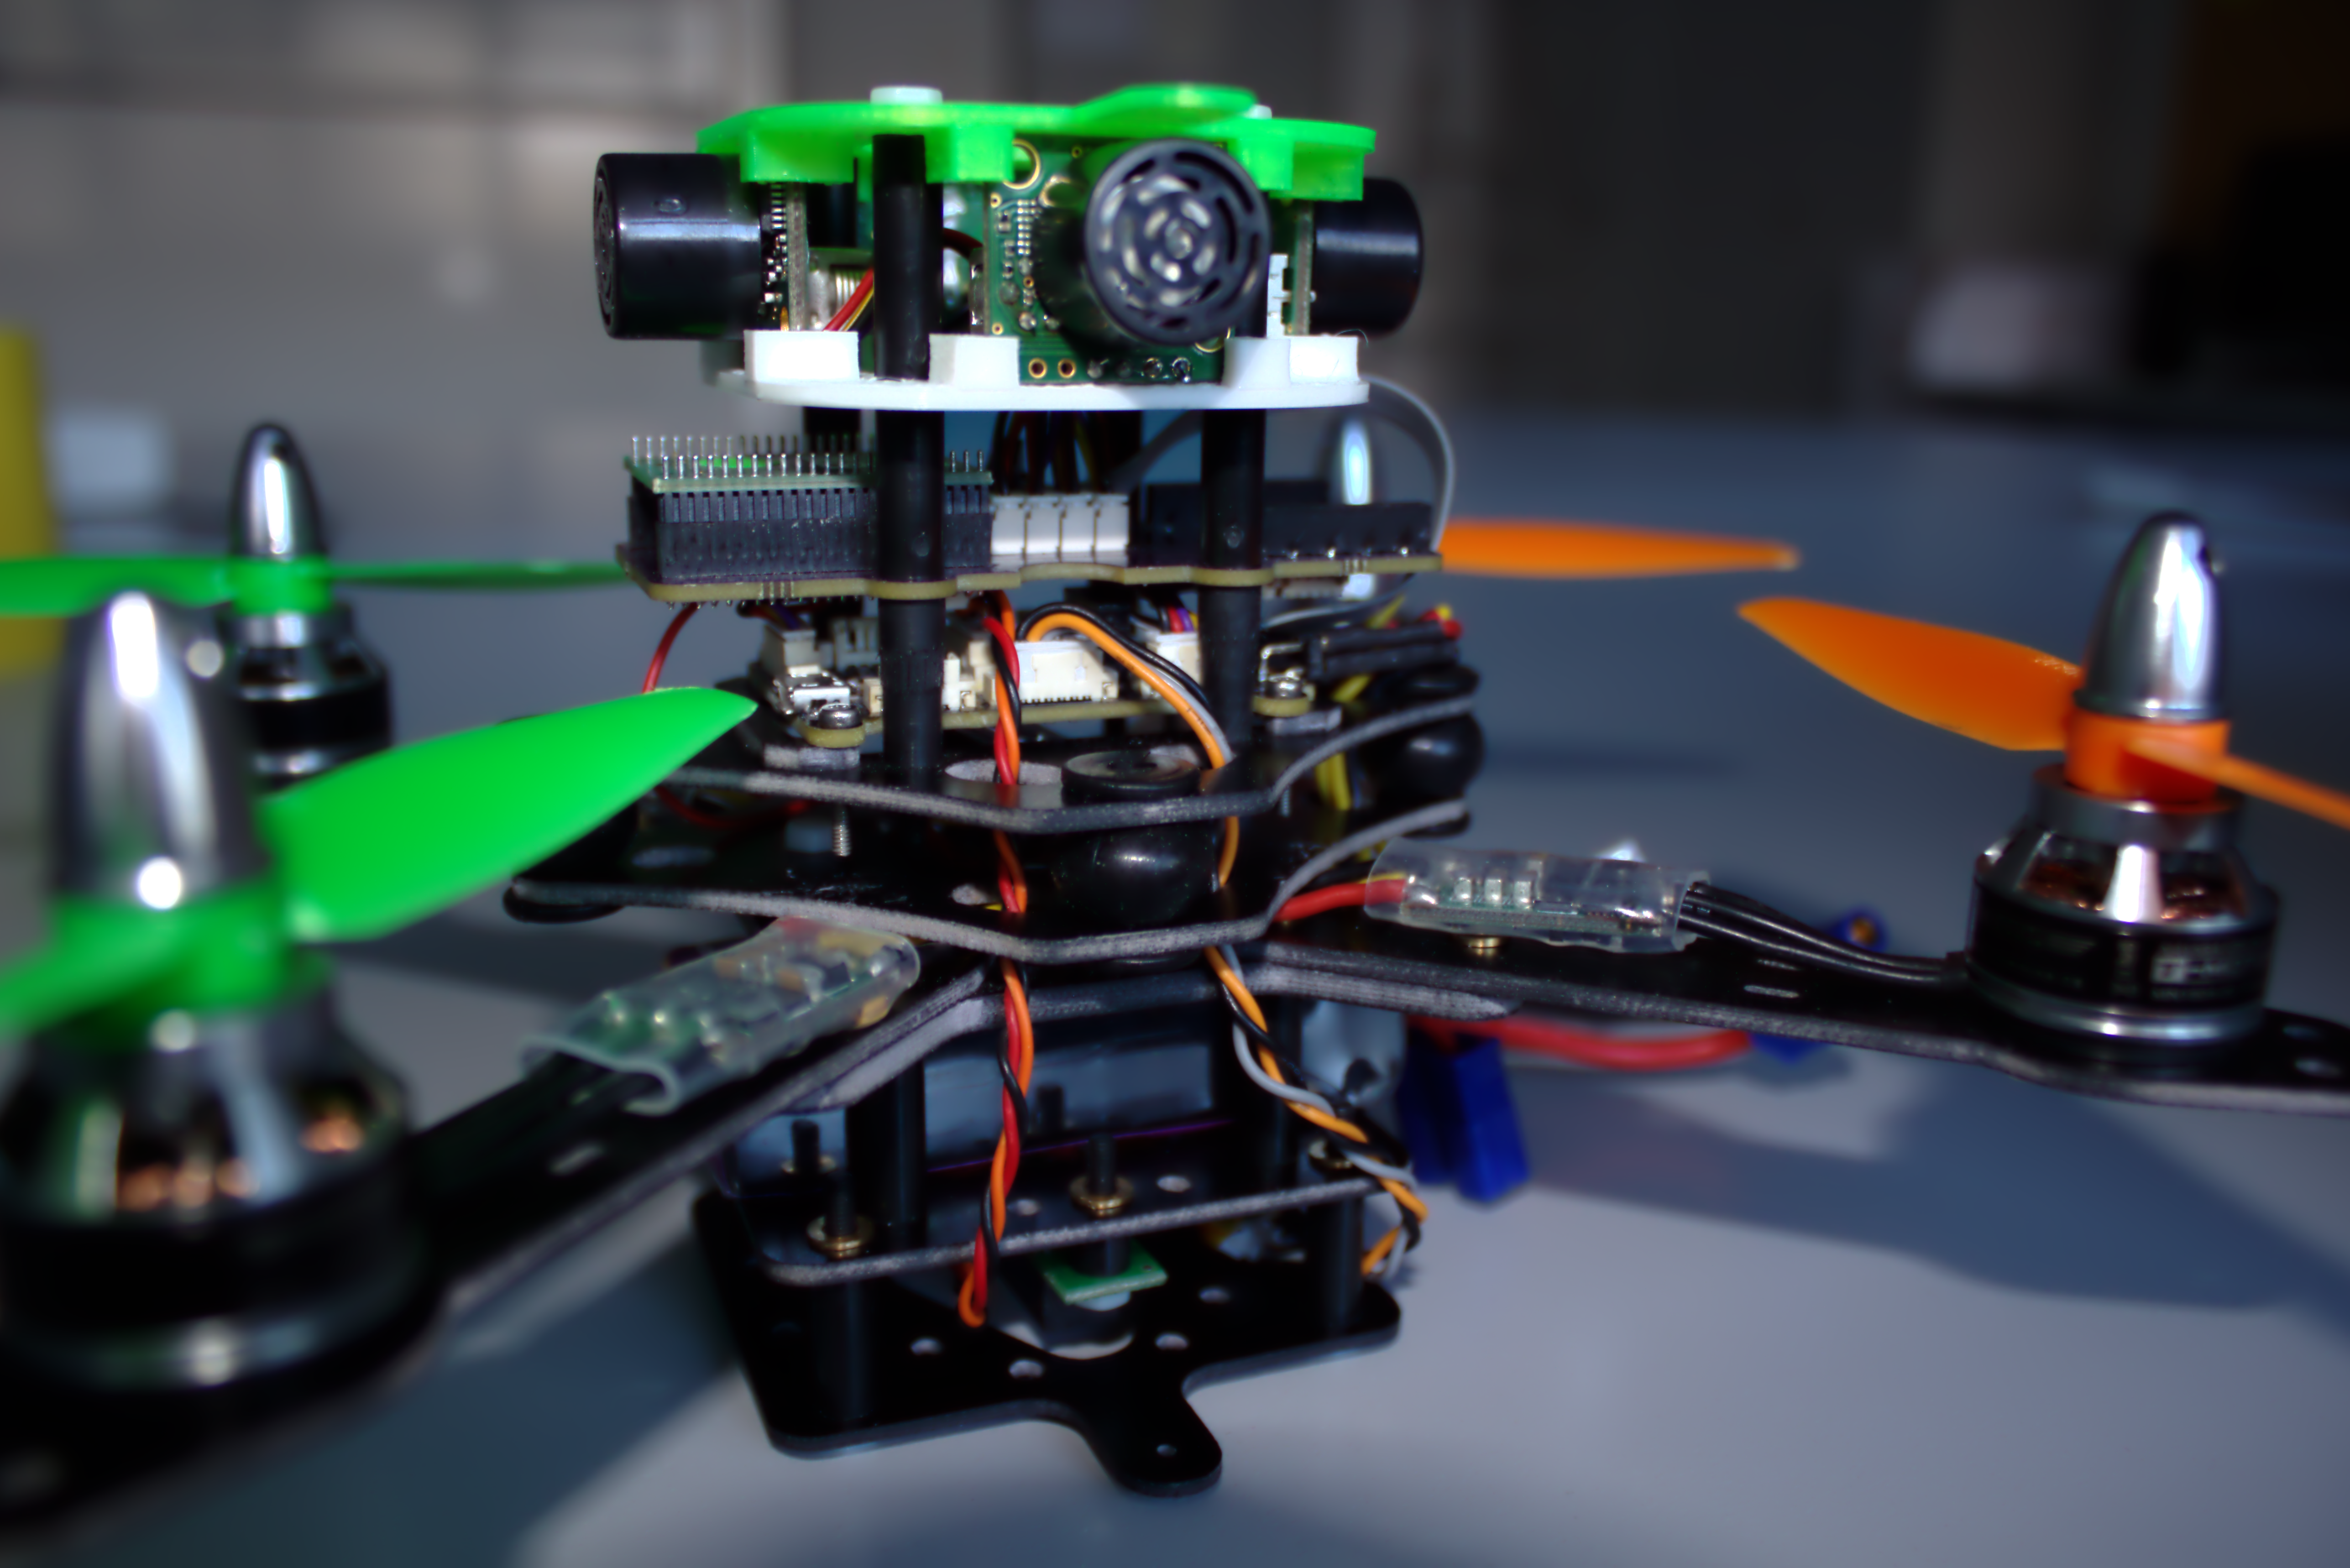
\includegraphics[width=0.9\textwidth]{figures/copter.png}
\label{copterfoto}
\caption{The FINken robot, revision 3}
\end{figure}

The robots are propelled by four rotors that are directly attached to a brushless motor.
In combination the motors can be controlled to change the direction of the thrustvector (pitch and roll), to change the overall amount of lift generated (thrust) and to change the orientation of the airframe (yaw).
The airframe houses all the actuators, processors and batteries needed for flight.
Additionally it carries a multitude of sensors used for operating autonomsly.

\todo{überleitung}

The robots are capable of highly dynamic flight maneuvers–the robots have enough acceleration to leave the operating environment in any possible direction in under one second.
This is mainly because the robots need lots of payload capacity to carry different sensors and computing power, with enough headroom to make changes in the future.
However the capability for dynamic beheaviour is not usefull for our research.
Of course the high power of the motors can also be used to stabilize the copter better, which is exactly what is needed for the FINken research.
If the copter is angled by only $6\degree$ and it's height is kept stable it is accelerating at about \SI{1}{\metre\per\square\second} if the height stays the same during that time.
This means the copter reaches a velocity of over \SI{2}{\metre\per\second} when travelling through the arena at this pretty small angle. \todo{kleine störung-> rel. großer effekt}

\subsection{Environment}
When doing research things do not always work perfectly.
Therefore the environment for the FINken robots is designed to protect the robots from mechanical damage.
It is also designed not to intefere with the function of the sensors the robot is using. 

The FINken robots fly in an area of \SI{2}{\metre} by \SI{3}{\metre} that can be expanded to about \SI{3}{\metre} by \SI{4}{\metre}.
The flight area is enclosed by netting and ultrasound-reflecting foil those barriers act the same way a wall would without damaging the robots if they fail to elude them.
Usually the altitude of operation is between \SI{0.5}{\metre} to \SI{1}{\metre}.
To prevent damage when the quadcopters crash the floor is coverd with mats that work well with ultrasound and infrared sensors.
It is possible to create virtual environmental factors by using a projector and an rgb-sensor mounted on top of the robots.
This virtual environment can be used research the beheaviour of the quadcopters if a certain task is assigned to the robot, e.g. finding the brightest spot.
\todo{foto}


\subsection{Sensor Concept}
The sensors used by the FINken robots serve two purposes: To enable the robots to fly autonomsly and to interact with other robots and the environment.

\subsubsection{Autonomous Flying}
To form a swarm the robots need to function as single individuals first-that means not crashing into walls, ceiling, floor or other robots.
Of course the sensors needed for autonoms flight must not be disturbed by the other componets of the quadcopter.

To simplify the control of the quadcopters no complex movements shall be made.
The robots shall be able to fly at a given height and navigate in x-y-direction to perform their given tasks.
%Highly dynamic maneuvers are possible for the airframe, but are not realizable with the sensor data we currently get. \todo{ref to christophs ba}
Flying autonomously like this requires to solve two major problems: Height control and navigation.

For controlling the height of the copters either the ultrasound distance measurement of the optical flow sensors are used, alternativly the height is measured by an infrared sensor that needs to be equipped when the optical flow sensors are not.

%The flight dynamics of the FINken robots shall be as simple as possible.

Navigating the x-y-plane is a much harder task.
Because sensors are not perfect the copter will drift in any given direction and precise speed and position measurements are lacking with the current sensor setup.
As a consequence implementing a position hold or navigation by waypoints is not possible.
Even without those navigation methods there is a well working strategie for flying for longer time periods.
With its ultrasound distance sensors the robot can sense its surroundings and is able to stay in the arena by maintaining a safe distance from the walls of the arena and other objects in the way. \todo{link to christophs ba}
An essential precondition for navigating around obstacles that way is avoiding highly dynamic maneuvers.

\subsubsection{Interaction}

The FINken robots shall be able to do more than randomly flying around without crashing.
The robot shall interact with its environment and it's neighbours in the swarm.
Of course sensor values needed for autonomous flight can also be used to interact with the robots environment, but there are also senors that are exclusively used for interaction.

To interact with it's environment the robot has different sensors.
The ultrasound distance sensors are used to measure distances to near objects.
However those sensors are not able to distinguish between those objects and are in this respect very different from the new ranging sensors.
To research interaction with an environment a solution is necessary to create a modifyable environmental factors that can be acted upon by the robots.
Those environmental factors shall be changed without altering the physical layout of the lab.
In the swarmlab a beamer is used to project an into the operating area.
The current lighting situation can be measured by an rgb color sensor that is mounted on top of the copter.

The new range sensor is also mainly used for interaction between the robots.
It can be used to create environmental input for exmple to probvide points of interest or to mark certain locations that shall be avoided by other quadcopters
Ranging values enable the FINken robots to interact with each other based on their distance i.e. by implementing attraction-repulsion-beheaviour. \todo{more?}

\subsection{Hardware Description}
There are different ranging technologies that might be used in a FINken quadcopter.
However there are different components that can interfere with the new sensor that shall be integrated e.g. by disturbing the measurments made by the new sensor.

%The FINken 3 robots are quadcopters controlled by the Lisa\/MX 2.1 autopilot-board\cite{_lisa/mx_????} using the opensource autopilot firmware Paparazzi\cite{_paparazziuav_????}.
\begin{table}[H]
	\begin{tabularx}{\columnwidth}{l | X}
	Part & Description \\ \hline
	Frame & The Frame is made of GFK material and plastic and rotor to rotor distance is \SI{10}{\centi\metre} \\
	Propellers & The FINken use \SI{5}{"}x\SI{3}{"} propellers \\
	Motors & Four brushless motors that may cause RF-interfercene and noise \\
	Power-Supply & Lithium polymer batteries with nominally \SI{11.1}{\volt} output voltage that is converted to 5V and 3.3V by the power distribution hardware \\
	Sonar Sensors & Sonar sensors to measure distances of the nearest object in four directions (front, back, left, right) \\
	Optical Flow & PX4 Optical flow sensor to measure x- and y- velocity and distance to ground \\
	IR-Sensor & IR-Distance sensor measuring distance to ground, alternativ to optical flow sensor \\
	Telemetry & BTLE-/Zigbee modules to exchange data with the ground station \\
	RC-Control &  2.4GHz based Radio Control to manually control the robots \\
	\end{tabularx}
	\caption{Hardware Components of the FIKen 3 robots}
\end{table}

\section{Evaluation of Existing Ranging Solutions}

\todo{mehr fokus auf andere copter projekte}
Keeping the requirements from \autoref{req} in mind  there are some technologies that can be used for ranging.
The usual application for most of those technologies in research is positioning, which makes it difficult to find comparable numbers for ranging-only applications.



It is still interesting to search for positioning applications, since many of those positioning technologies are based on multilateration\footnote{The usual methods for positioning are: \emph{multilateral}—which is what we are interested in because only ranging measurments are used, \emph{multiangular}—which is no use  to us, because angle measurements are used and by \emph{orientating in a map} with different factors like beacon-positions–which is also no use to us.}.
\cite{_multilateration_2015}
\todo{keep it or throw it away?}

\subsection{Optical Tracking}

Most projects use external optical tracking to measure the position and orientation of the quadcopters. \todo{refs}

The most common optical tracking systems are very costly in comparison to the other ranging methods described here.
The most affordable solution from Optitrack that is able to track 5 targets at once costs more then \SI{10000}{\$}\cite{optitrack.com}.
The price is justified by the superior performance of this method.
This means tracking accuracy as well as the possibility to measure orientation at a very high update frequency.
\todo{research performance statistics for ranging solutions}

\todo{ETH}

However this approach is exactly the multi agent systems approach to provide global knowlegde that has been gathered by the tracking system to the agents in contrast to swarm beheaviour that is relying on local information.
The biggest drawback of this approach is that we gather global knowledge about our system, rather than creating beheaviour based on local interaction.
As such external tracking would be a valuable tool for evaluation, but is not meeting the requirements for gathering sensor data.

%A huge drawback to this method is that many components are used that need to be integrated into the environment and cannot be carried by the robots themselves.
%For swarm robotics this is not an ideal solution as using external tracking would mean communicating with some kind of centralized tracking interface-destroying the scalability and the priciple of local interaction leading to global beheaviour.

\subsection{Indor Time of Flight}
An obvious approach for replacing the GPS signal is to use a simmilar approach indoors.

The problem is that very short timespans have to be measured accuratly, because radio waves are so damn fast. \todo{wording}
\cite{lanzisera2006} states, that standard errors of \SI{2.6}{\metre_{RMS}} and \SI{1.8}{\metre_{RMS}} was measured in different indoor scenarios.
With an operating area only \SI{3}{\metre} wide this approach is not suited for our robots.


% \cite{uwb_decawave} claims that an accuracy of \SI{10}{\centi\metre} can be achieved and the nodes are aviable for purchase at reasonable prices. \todo{begründen warum wir das nicht benutzen} \todo{wiederspruch mit den 10cm, more like 50cm}
A project that looks more promising is decaWave.
According to \cite{uwb_localisation_copter} the measurement error is generally under \SI{1}{\metre} and with filtering can be brought to below \SI{15}{\centi\metre}.
The proposed method of filtering needs 27 measurements to compute one range value.\todo{wording}
However the decaWave project was unkown to us when we started looking for ranging possibilities so \todo{blabla}

\subsection{Ultrasonic Time of Flight Ranging}
A very clever approach to ranging is used by ranging solutions like cricket~\cite{cricket_01} and active bat~\cite{active_bat}. 
RF-Signals travel at the speed of light and therefore very short time-periods need to be measured accurately to compute distances from time of flight.
Sound however travels at a speed much slower than radio waves so the time periods that need to be measured are much longer.
Infact the time periods get so long that another problem comes up.

Using sound as medium there is an upper bound to the update frequency for all nodes sharing the medium (i.e. close enough to sense each other).~\cite{active_bat} claims that one ranging measurement can be done in a \SI{20}{\milli\second} slot.
That means we can have 50 range updates per second. Assuming we have a swarm of five robots that form a fully connected graph we would need at least ten range measurements to get all swarm distances.
So the upper boundary for ranging update frequency in a swarm of five robots is \SI{5}{\hertz}.
Considering that this is the upper limit this is a solid disadvantage of this method.
Furthermore the FINken robots currently use sonar based distance sensor to measure the distance to the nearest object in some direction so either the update frequency would be diminished much further.

%Another problem is the noise created by motors and propellers.
%The sound made by the quadcopters is not ending in the hearable spectrum but also extends to the ultrasound range.
In conclusion ultrasound based ranging is a very neat approach to ranging that is already used in other quadcopter projects~\cite{ultrasonic_erlangen}.
Still integrating an ultrasonic ranging sensor into the FINken is impractical, because other ultrasound sensors are already in use.
%\todo{accuracy / price, moving objects}


\subsection{Signal Strength}

A property that can be used to do RF-based ranging is signal strength.
The further the source of the signal is away the weaker the signal gets.
RSSI\footnote{Received Signal Strength Indicator}-based ranging is done for serveral different wireless technologies: Bluetooth\todo{quelle}, WLAN\todo{quelle}, RFID\todo{quelle} –
There are even approaches using maps composed of different RSSI-ranging values. http://www.gnss.com.au/JoGPS/v9n2/JoGPS\_v9n2p122-130.pdf \todo{quellify}

The main factor that rules out RSSI-based ranging is that radio-waves are not propageted equally in every direction. \todo{typical propagation pattern picture}
As a consequence the orientation of the antenna might have a much bigger impact on signal strength then the distance.
Additionally radio waves might be weakend when travelling through the FINken robots.

\subsection{Atmel RTB, Dresden Elektronik, Meterionic}

Another thing that can be measured phase shift.
This is a principle that is used by some of the ultrasonic methods.
However the phase difference can also be measured in radio waves.
This is utilized by the ranging hardware from the Atmel Ranging Toolbox.
Multiple frequencys are used to measure a phase difference.
Because the wave length changes with different frequencys you can take all of the measured phase differences and compute a distance.
\todo{quelle}
Similar hardware using the same software stack is also sold by \emph{Dresden Elektronik} and \emph{Meterionic}.

Using phase differences in RF discards the medium access problems of ultrasonic methods as well as the wave propagation problems of RSSI-based methods.
Therefore it seems like a feasible approach for the FINken robots.

